\subchapter{Bootloader - U-Boot}{Objectives: Set up serial
  communication, compile and install the X-Loader and U-Boot
  bootloaders, use basic U-Boot commands, set up TFTP communication
  with the development workstation.}

As the bootloader is the first piece of software executed by a
hardware platform, the installation procedure of the bootloader is
very specific to the hardware platform. There are usually two cases:

\begin{itemize}

\item The processor offers nothing to ease the installation of the
  bootloader, in which case the JTAG has to be used to initialize
  flash storage and write the bootloader code to flash. Detailed
  knowledge of the hardware is of course required to perform these
  operations.

\item The processor offers a monitor, implemented in ROM, and through
  which access to the memories is made easier.

\end{itemize}

The IGEPv2 board, which uses the DM3730 or the OMAP3530 processors, falls into
the second category. The monitor integrated in the ROM reads the MMC/SD
card to search for a valid bootloader before looking at the internal
NAND flash for a bootloader. Therefore, by using an MMC/SD card, we can
start up a OMAP3-based board without having anything installed on it.

\section{Setup}

Go to the \code{/home/<user>/felabs/sysdev/u-boot/} directory.

\section{MMC/SD card setup}

The ROM monitor can read files from a FAT filesystem on the MMC/SD
card. However, the MMC/SD card must be carefully partitionned, and the
filesystem carefully created in order to be recognized by the ROM
monitor. Here are special instructions to format an MMC/SD card
for the OMAP-based platforms.

First, connect your card reader to your workstation, with the MMC/SD
card inside. Type the \code{dmesg} command to see which device is used
by your workstation. Let's assume that this device is \code{/dev/sdb}.

\begin{verbatim}
sd 3:0:0:0: [sdb] 3842048 512-byte hardware sectors: (1.96 GB/1.83 GiB)
\end{verbatim}

\fbox{\begin{minipage}{\textwidth}
{\bfseries
Caution: read this carefully before proceeding. You could destroy
existing partitions on your PC!

Do not make the confusion between the device that is used by your
board to represent your MMC/SD disk (probably \code{/dev/sda}), and the device
that your workstation uses when the card reader is inserted (probably
\code{/dev/sdb}).

So, don't use the \code{/dev/sda} device to reflash your MMC disk from
your workstation. People have already destroyed their Windows
partition by making this mistake.}
\end{minipage}}

You can also run \code{cat /proc/partitions} to list all block devices
in your system. Again, make sure to distinguish the SD/MMC card from the
hard drive of your development workstation!

Type the \code{mount} command to check your currently mounted
partitions. If MMC/SD partitions are mounted, unmount them:

\begin{verbatim}
$ sudo umount /dev/sdb1
$ sudo umount /dev/sdb2
...
\end{verbatim}

Now, clear possible MMC/SD card contents remaining from previous training 
sessions:

\begin{verbatim}
$ sudo dd if=/dev/zero of=/dev/sdb bs=1M count=256
\end{verbatim}

As we explained earlier, the TI OMAP rom monitor needs special partition geometry settings
to read partition contents. The MMC/SD card must have 255 heads and 63 sectors.

Let's use the \code{cfdisk} command to create a first partition with these settings:

\code{cfdisk -h 255 -s 63 /dev/sdb}

In the \code{cfdisk} interface, create a first primary partition, starting from the beginning,
with a 64 MB size, a \code{Bootable} type and a \code{0C} type (\code{W95 FAT32 (LBA)}).
Press \code{Write} when you are done.

If you used \code{fdisk} before, you should find \code{cfdisk} much more convenient!

Format this new partition in FAT32, with the \code{boot} label (name):

\begin{verbatim}
sudo mkfs.vfat -n boot -F 32 /dev/sdb1
\end{verbatim}

Then, remove and insert your card again.

Your MMC/SD card is ready to use.

\section{X-loader setup}

Download the X-loader source code from the IGEP support Git
repository:\footnote{We are using an old version of X-Loader, because
  the most recent versions provided by ISEE have been modified to use
  a completely non-standard boot procedure, that we don't think is
  interesting to present in a training session. The new ISEE boot
  procedure places the kernel image inside a JFFS2 filesystem, and
  completely bypasses U-Boot. This is not standard, and the procedure
  with two bootloaders presented below is much more common at the
  moment on most embedded platforms.}

\begin{verbatim}
sudo apt-get install git
git clone git://git.igep.es/pub/scm/x-loader.git
cd x-loader
git checkout v1.4.4-3
\end{verbatim}

Then, we need to apply a {\em patch} that adds NAND support to
X-Loader:

\begin{verbatim}
cat ../x-loader-1.4.4-3-igep-nand-support.patch | patch -p1
\end{verbatim}

In order to compile the X-loader, you need to:
\begin{itemize}

\item set the \code{CROSS_COMPILE} environment variable:\\
\code{export CROSS_COMPILE=arm-linux-}

\item specify the \code{PATH} to the toolchain that you made:\\
\code{export PATH=/usr/local/xtools/arm-unknown-linux-uclibcgnueabi/bin:$PATH}

\item run \code{make igep0020-sdcard_config} to set the configuration
  for the target board.

\item run \code{make} to build the image

\end{itemize}

The resulting file is stored in the \code{x-loader} main directory as
\code{x-load.bin}. This file must be {\em signed}\footnote{In fact,
  for a General Purpose (GP) device, the signature only consists of
  adding a “Table of Contents” at the beginning of the image,
  explaining which program to execute. Signatures are using in variants
  of the OMAP CPUs that implement some security features, which will refuse
  to load an X-loader image that wasn't signed with an authorized key.}
  in order to be executed by the processor. Using the \code{signGP} tool in the \code{contrib/}
subdirectory, sign the \code{x-load.bin} file:

\begin{verbatim}
./contrib/signGP x-load.bin
\end{verbatim}

This produces an \code{x-load.bin.ift} file. You can copy it to the
MMC card, renaming it as \code{MLO}.

\section{U-Boot setup}

Download U-Boot from the mainline igep download site:

\begin{verbatim}
wget ftp://ftp.denx.de/pub/u-boot/u-boot-2011.12.tar.bz2
tar xvf u-boot-2011.12.tar.bz2
cd u-boot-2011.12
\end{verbatim}

Now we need to apply a patch to add NAND support for the IGEP board:

\begin{verbatim}
cat ../u-boot-2011.12-igep-nand-support.patch | patch -p1
\end{verbatim}

Get an understanding of its configuration and compilation steps by
reading the \code{README} file, and specifically the {\em Building the
  software} section.

Basically, you need to:

\begin{itemize}

\item set the \code{CROSS_COMPILE} environment variable (you should
  have already done it when you compiled X-loader);

\item run \code{make <NAME>_config}, where \code{<NAME>} is the name
  of a configuration file in \code{include/configs/}. For our
  platform, the configuration file is
  \code{include/configs/igep0020.h}. Read this file to get an idea of
  how a U-Boot configuration file is written;

\item Finally, run \code{make}\footnote{You can speed up the compiling
  by using the \code{-jX} option with \code{make}, where X is the number of parallel
  jobs used for compiling. Twice the number of CPU cores is a good
  value.}, which should build U-Boot.

\end{itemize}

You can now copy the generated \code{u-boot.bin} file to the MMC card.

Unmount the MMC card partition.

\section{Setting up serial communication with the board}

Plug the IGEPv2 board on your computer using the provided
USB-to-serial cable. When plugged-in, a serial port should appear,
\code{/dev/ttyUSB0}.

You can also see this device appear by looking at the output of
\code{dmesg}.

To communicate with the board through the serial port, install a
serial communication program, such as \code{picocom}:

\begin{verbatim}
sudo apt-get install picocom
\end{verbatim}

Run \code{sudo picocom -b 115200 /dev/ttyUSB0}, to start serial
communication on \code{/dev/ttyUSB0}, with a baudrate of 115200. If
you wish to exit picocom, press \code{[Ctrl][a]} followed by
\code{[Ctrl][x]}.

\section{Testing U-Boot on the MMC card}

Insert the MMC card into the IGEP board, reset the board and check
that it boots your new bootloaders. You can verify this by checking
the build dates:

\begin{verbatim}
Texas Instruments X-Loader 1.4.4-3 (May  4 2012 - 10:26:41)
CPU Release: 0x2b89102f - 0x2
XLoader: CPU status = 0xe00
XLoader: Processor DM3730 - ES1.2
XLoader: Memory Manufacturer: Micron (2c)
Loading u-boot.bin from mmc


U-Boot 2011.12 (May 04 2012 - 10:31:05)

OMAP36XX/37XX-GP ES1.2, CPU-OPP2, L3-165MHz, Max CPU Clock 1 Ghz
IGEP v2 board + LPDDR/ONENAND
I2C:   ready
DRAM:  512 MiB
NAND:  512 MiB
MMC:   OMAP SD/MMC: 0
In:    serial
Out:   serial
Err:   serial
Die ID #1bd600029ff80000016842c80f03400d
Net:   smc911x-0
Hit any key to stop autoboot:  3
\end{verbatim}

By the message {\em Loading u-boot.bin from mmc} you also get the
confirmation that your U-Boot has correctly been loaded from the MMC
device.

Interrupt the countdown to enter the U-Boot shell:
\begin{verbatim}
U-Boot #
\end{verbatim}

In U-Boot, type the \code{help} command, and explore the few commands available.

\section{Reflashing from U-boot}

We will first reflash the X-Loader in NAND. To do so, type the following commands:

\begin{verbatim}
mmc rescan
\end{verbatim}

This initializes the MMC interface

\begin{verbatim}
fatload mmc 0 81000000 MLO
\end{verbatim}
This loads the file from MMC 0 partition 0 to memory at address 0x81000000

\begin{verbatim}
nandecc hw
\end{verbatim}

This tells U-Boot to write data to the NAND using the hardware ECC
algorithm, which the ROM code of the OMAP uses to load X-Loader.

\begin{verbatim}
nand erase 0 80000
\end{verbatim}

This command erases a 0x80000 byte long space of the NAND flash from offset 0

\begin{verbatim}
nand write 81000000 0 80000
\end{verbatim}

This command writes data to the NAND flash. The source is 0x81000000
(where we've loaded the file to store in the flash) and the
destination is offset 0 of the NAND flash. The length of the copy is
0x80000 bytes, which corresponds to the space we've just erased
before. It is important to erase the flash space before trying to
write on it.

X-Loader has been transfered to NAND flash. You can now do the same
with U-Boot.  The storage offset in the NAND is 0x80000 (just after
the space reserved for X-Loader) and the length is 0x180000. You will
have to flash U-Boot to NAND with the software ECC algorithm, which
X-Loader uses to load U-Boot from NAND. This can be achieved by
running the \code{nandecc sw} command.

After flashing the U-Boot image, also erase the U-boot environment
variables defined by the manufacturer or by previous users of your
board:

\begin{verbatim}
nand erase 200000 80000
\end{verbatim}

You can remove MMC card, then reset the IGEP board. You should see the
freshly flashed X-Loader and U-Boot starting.

You should now see the U-Boot prompt:

\begin{verbatim}
U-Boot #
\end{verbatim}

\section{Setting up Ethernet communication}

Later on, we will transfer files from the development workstation to
the board using the TFTP protocol, which works on top of an Ethernet
connection.

To start with, install and configure a TFTP server on your development
workstation, as detailed in the bootloader slides.

With a network cable, connect the Ethernet port of your board to the
one of your computer. If your computer already has a wired connection
to the network, your instructor will provide you with a USB Ethernet
adapter. A new network interface, probably \code{eth1} or \code{eth2},
should appear on your Linux system.

To configure this network interface on the workstation side, click on
the {\em Network Manager} tasklet on your desktop, and select {\em
  Edit Connections}.

\begin{center}
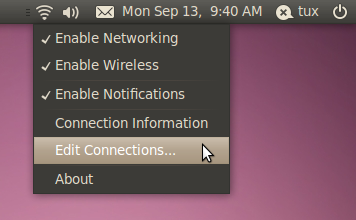
\includegraphics[width=8cm]{labs/sysdev-u-boot/network-config-1.png}
\end{center}

Select the new {\em wired network connection}:

\begin{center}
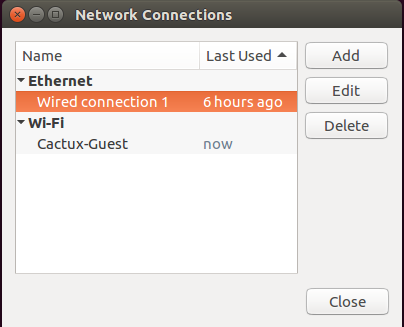
\includegraphics[width=8cm]{labs/sysdev-u-boot/network-config-2.png}
\end{center}

In the {\em IPv4 Settings} tab, make the interface use a static IP
address, like \code{192.168.0.1} (of course, make sure that this
address belongs to a separate network segment from the one of the main
company network).

\begin{center}
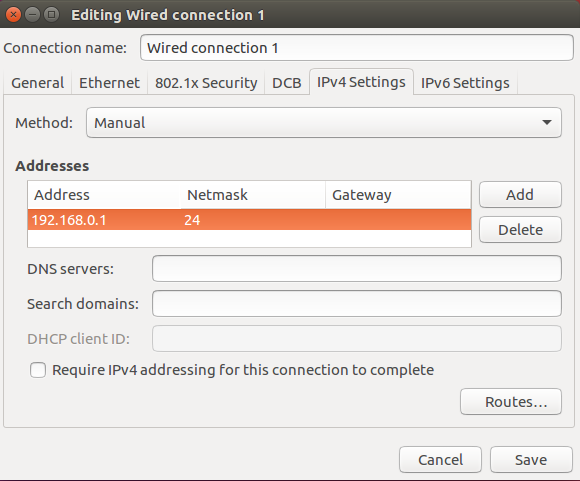
\includegraphics[width=8cm]{labs/sysdev-u-boot/network-config-3.png}
\end{center}

You can use \code{255.255.255.0} as \code{Netmask}, and leave the
\code{Gateway} field untouched (if you click on the \code{Gateway} box, you
will have to type a valid IP address, otherwise you won't be apply to
click on the \code{Apply button).

Now, configure the network on the board in U-Boot by setting the \code{ipaddr}
and \code{serverip} environment variables:

\begin{verbatim}
setenv ipaddr 192.168.0.100
setenv serverip 192.168.0.1
\end{verbatim}

In case the board was previously configured in a different way, we
also turn off automatic booting after commands that can be used to
copy a kernel to RAM:

\begin{verbatim}
setenv autostart no
\end{verbatim}

In case it is not set yet, you may also need to configure the MAC address for the board:

\begin{verbatim}
setenv ethaddr 01:02:03:04:05:06
\end{verbatim}

To make these settings permanent, save the environment:

\begin{verbatim}
saveenv
\end{verbatim}

Now switch your board off and on again\footnote{Power cycling your
  board is needed to make your ethaddr permanent, for obscure
  reasons. If you don't, U-boot will complain that ethaddr is not
  set.}.

You can then test the TFTP connection. First, put a small text file in
the directory exported through TFTP on your development
workstation. Then, from U-Boot, do:

\begin{verbatim}
tftp 0x80000000 textfile.txt
\end{verbatim}

This should download the file \code{textfile.txt} from your development
workstation into the board's memory at location 0x80000000 (this
location is part of the board DRAM). You can verify that the download
was successful by dumping the contents of the memory:

\begin{verbatim}
md 0x80000000
\end{verbatim}

We will see in the next labs how to use U-Boot to download, flash and
boot a kernel.
